%% UniMind -- IEEE Transactions on Computers submission draft (v2)
%% Two-column IEEEtran journal format. Target 11-14 pp.
\documentclass[journal,10pt,twocolumn]{IEEEtran}

\usepackage{cite}
\usepackage{amsmath,amssymb}
\usepackage{graphicx}
\usepackage{booktabs}
\usepackage{array}
\usepackage{multirow}
\usepackage{xcolor}
\usepackage{pgfplots}
\pgfplotsset{compat=1.17}
\pgfplotsset{every axis/.append style={font=\footnotesize}}
\usepackage{url}
\usepackage{algorithm}
\usepackage{algpseudocode}
\usepackage{ragged2e}
\usepackage{microtype}
\usepackage{enumitem}
\usepackage{tikz}
\usetikzlibrary{arrows.meta,positioning}
\usepackage[hidelinks]{hyperref}

\newcommand{\q}[1]{\texttt{q#1}}
\newtheorem{definition}{Definition}

\hypersetup{pdftitle={UniMind: Calibration-Aware Scheduling and Placement for Quantum-Accelerated AI Middleware},
            pdfauthor={Y. X. Tan}}

\begin{document}

\title{UniMind: Calibration-Aware Scheduling and Placement for Quantum-Accelerated AI Middleware}

\author{Y.~X.~Tan%
\thanks{Y.~X.~Tan is an independent researcher (e-mail: yxtan5022@gmail.com). All experiments are open-source and
reproducible from \texttt{yxtan5022-maker/unimind-v2}; QPU job IDs and snapshots are recorded in the data directory.}}

\markboth{Transactions on Computers,~Vol.~XX, No.~XX, Month~Year}%
{Author \MakeLowercase{\textit{et al.}}: UniMind: Calibration-Aware Scheduling and Placement}

\maketitle

% ---------------------------------------------------------------- Abstract
\begin{abstract}
Quantum-accelerated AI workloads must be scheduled onto physical devices whose calibration changes
between runs. A classical scheduler assumes resources are identical and stable; a quantum scheduler
faces an array of qubits whose individual noise parameters drift daily. This paper asks:
\emph{how should a quantum runtime maintain scheduling decisions when hardware calibration changes
over time?} We instrument a 156-qubit superconducting device across three daily calibration
snapshots (D0--D2; 2026-08-29 to 08-31) and build \textbf{UniMind}, a middleware that scores,
places, executes, and refreshes calibration data in a closed loop. Three findings are established:
\textbf{(1)~Calibration validity is temporally bounded.} Day-over-day rank correlation is only
$\rho{=}0.579$, top-10 overlap is $0.25$, and a stale top-3 pin is $2.1\times$ worse than a fresh
selection within 24~h. We formalize the \emph{Calibration Validity Horizon}
$T_{\mathrm{valid}}$: the time window over which a calibration-derived placement remains within
fidelity tolerance. \textbf{(2)~Adaptive refresh beats static and periodic policies.} A two-line
trigger (top-10 Jaccard $<0.5$ or $\Delta C{>}0.005$) detects staleness at near-zero cost
($\sim0.04$~ms per scoring pass). Offline threshold sweeps over $\tau_J{\in}[0.1,0.9]$ and
$\tau_C{\in}[0.001,0.02]$ reveal the Pareto tradeoff between refresh rate and fidelity;
the measured trigger sits near the knee. \textbf{(3)~Refresh, not placement selection, dominates
end-to-end reliability.} Fresh pins lift \emph{both} the pinned and free arms by $+33/37$~pp on a
6-qubit angle suite; the pinned vs.\ free difference is within noise ($70.0\%$ vs.\ $76.7\%$,
$p{=}0.56$). A negative result completes the picture: re-fitting the 7-dim layout utility $J(G)$
on real device labels collapses its out-of-sample Spearman from $\rho{=}0.818$ to $0.13$
($p{=}0.36$), because the simulator proxy over-penalizes large layouts that a refresh-pinned
device does not. We give the validity model, the measured numbers, the adaptive mechanism, and
the explicit negative results.
\end{abstract}

\begin{IEEEkeywords}
quantum computing middleware, calibration-aware scheduling, calibration validity horizon, adaptive refresh,
qubit placement, calibration drift, resource management, quantum-cloud runtime, reliability composition.
\end{IEEEkeywords}

% ---------------------------------------------------------------- Intro
\section{Introduction}
\IEEEPARstart{E}{mbedded} AI is increasingly offloaded to accelerator hardware, and quantum processors are the
newest such accelerator. Their software stack, however, changes the \emph{scheduler's} job in a fundamental way: a
quantum circuit's fidelity depends on \emph{which} physical qubit executes it and \emph{when} that qubit was last
calibrated~\cite{preskill2018,arute2019,murali2019noise,li2019sabre}. A classical scheduler assumes resources are
identical and stable; a quantum scheduler faces an array of hundreds of qubits whose individual noise parameters
move between runs~\cite{ibmcalib,kanazawa2021,vanberg2023}.

Quantum-machine-learning (QML) frameworks---PennyLane~\cite{berholm2018}, Qiskit~\cite{qiskit}, TensorFlow
Quantum---provide algorithm abstractions but not the \emph{system} layer: dynamic backend discovery, layout
selection, and calibration refresh. Applications are assumed, usually silently, to have been placed on ``good
enough'' qubits. On real devices this assumption fails measurably: with \emph{free} transpiler placement an
angle-encoding experiment on \texttt{ibm\_marrakesh} missed the $0.05$ fidelity tolerance by up to $0.392$,
while the \emph{same} circuits on a pinned calibrated layout passed everywhere (max.\ deviation $0.028$)
\cite{tangpu}. Placement is not cosmetic; it is the dominant accuracy term at our test scale.

This paper addresses the temporal dimension of that problem. Placement decisions are made from a calibration
snapshot, and snapshots change daily; the scheduler's real questions are ``\emph{how old is my snapshot}'' and
``\emph{should I refresh}'' as much as ``\emph{where to place}''. We define the \textbf{Calibration Validity
Horizon} $T_{\mathrm{valid}}$: the maximum age of a calibration snapshot such that the resulting placement
remains within fidelity tolerance. With $T_{\mathrm{valid}}$ small (hours, not days), the runtime must refresh
frequently; with $T_{\mathrm{valid}}$ large, refresh is wasteful. We measure $T_{\mathrm{valid}}$'s lower bound
on a 156-qubit device across three daily snapshots, design an adaptive refresh trigger that detects staleness at
near-zero cost, and show that refresh---not placement selection---is where reliability engineering should invest.

This paper makes three contributions, all measured on a 156-qubit \texttt{ibm\_marrakesh} device across three
daily calibration snapshots (D0--D2; 2026-08-29 to 08-31):
\begin{enumerate}[leftmargin=1.8em,itemsep=1pt,topsep=2pt]
\item \textbf{Temporal validity analysis.} We quantify day-over-day calibration drift
($\rho{=}0.579$, $\tau{=}0.431$, top-10 Jaccard $0.25$), measure the staleness cost of aged pins
(stale top-3 is $2.1\times$ worse than fresh within 24~h), and formalize the Calibration Validity
Horizon $T_{\mathrm{valid}}$ as a design primitive for quantum runtimes (\S\ref{sec:drift}).
\item \textbf{Adaptive refresh policy.} We design a trigger (Jaccard $<0.5$ or $\Delta C{>}0.005$)
that detects staleness at near-zero cost, run offline threshold sweeps over $\tau_J$ and $\tau_C$ to
reveal the refresh-rate-vs.\-fidelity Pareto tradeoff, and compare static, periodic, and adaptive
policies on the same data (\S\ref{sec:drift}, \S\ref{sec:e2e}).
\item \textbf{Negative results.} The 7-dim layout utility $J(G)$, trained on a simulator proxy and
re-fitted on real device labels, collapses from out-of-sample $\rho{=}0.818$ to $0.13$
($p{=}0.36$); at $k{=}6$ with fresh pins, pinned placement shows no measured advantage over the
free transpiler ($70.0\%$ vs.\ $76.7\%$, $p{=}0.56$). We report these as bounds on what placement
engineering can deliver without temporal control (\S\ref{sec:jreal}, \S\ref{sec:e2e}).
\end{enumerate}

\noindent\textbf{Scope.} We make no claim of quantum advantage, novel quantum algorithms, or a production runtime.
We propose $T_{\mathrm{valid}}$ as a design primitive; with three daily snapshots we establish its lower bound and
demonstrate the adaptive mechanism, but leave the full multi-day decay curve and cross-device generalization to
future work. Every quantitative claim traces to a recorded job or snapshot; where an exploratory result did
not replicate (a first run's perfect rank correlation, $\rho{=}1.000$, which a fixed-design replication returned as
$\rho{=}0.771$, $p{=}0.103$) we report it with its failure. UniMind also contains an LLM-orchestration layer whose
reliability composition we \emph{do} model exactly (\S\ref{sec:calculus}), but the LLM's quality is a controlled
parameter of our experiments, never a claim about real models.

% ---------------------------------------------------------------- Background
\section{Problem and Related Work}
\subsection{Formal model}
\begin{definition}[Calibration-aware scheduling problem]
A device is a set of qubits $Q$ and couplers $E$ with a calibration snapshot $S_t$ reporting, per qubit, readout
assignment errors $(p_{0|1},p_{1|0})$, gate errors, and coherence times $(T_1,T_2)$. A job is a logical circuit
$\hat{G}$ over $k$ logical qubits. The scheduler chooses a \emph{placement} $\pi:\hat{G}\to Q$ (with
$|\pi|=k$, connected in $(Q,E)$ for our chains), a transpiler configuration, and a \emph{snapshot age policy}
that decides when $S_t$ is re-fetched. Its objective, subject to placement, snapshot age, and overhead budgets, is
per-qubit measurement fidelity $\max_i|Z_i^{\mathrm{emp}}\!\!-\!Z_i^{\mathrm{th}}|\!\le\!\epsilon$ at a
reliability target.
\end{definition}
The distinctness from classical placement lies in $(Q,E,S_t)$ being jointly non-stationary: $\pi$ chosen at time $t$
is evaluated at execution time $t'>t$ against a changed $S_{t'}$. The paper's arithmetic is about the size of that
violation.

\subsection{Related work}
\textbf{Placement and compilation.} Qubit mapping has both heuristic and exact treatments: SABRE~\cite{li2019sabre}
and noise-adaptive mappings~\cite{murali2019noise} fold device error into the routing pass; exact synthesis is
practical for small circuits~\cite{tan2020iccado}; resource-aware timing variants exist for heterogeneous
devices~\cite{lao2022timing}. Our contribution is not a new routing algorithm but \emph{who decides}: a middleware
layer that computes an \texttt{initial\_layout} from a score over a live snapshot and composes with any downstream
transpiler, plus an explicit staleness contract---aspects the compiler literature treats as ``the backend's
problem''.

\textbf{Error mitigation.} Measurement twirling~\cite{nation2023,bravyi2021meas}, probabilistic error cancellation,
and sparse Pauli--Lindblad models~\cite{vanberg2023,temme2017} correct errors statistically at shot cost. Our results
bound where mitigation is needed: it helps the \emph{broken} qubit and is redundant on the good one
(\S\ref{sec:placement}), which argues for calibration-conditional mitigation---a placement decision, not a
post-processing one.

\textbf{Runtime and cloud middleware.} Qiskit Runtime~\cite{ibmrtime}, Braket~\cite{braket}, and Azure
Quantum~\cite{azureq} manage jobs and queue bounds but expose placement as an option, not as a scheduler resource;
much of the practical ``does this job need mitigation, where, and with which snapshot'' knowledge lives in operator
runbooks. We know of no published quantified day-scale ranking drift for a 156-qubit device; the public signals
closest to it are per-device aggregate fidelities in documentation~\cite{ibmcalib} and in error-rate studies of
specific devices~\cite{kim2023utility}. We present the first measurements of the drift and the protocol (trigger,
refit-on-real-labels) that a runtime can adopt.

% ---------------------------------------------------------------- System
\section{UniMind Middleware}
\label{sec:architecture}
UniMind is a user-space, multi-backend middleware (Qiskit/Aer, CUDA-Q~\cite{cuquantum} via Qiskit, IBM Quantum).
Its scheduling core is the calibration-aware loop of Fig.~\ref{fig:loop}: one snapshot per calibration cycle,
$C(q)$ scoring, chain/utility placement, execution, and a refresh trigger. Two supporting layers are described
briefly. The \emph{orchestrator} interprets a task intent into candidate code under sandboxed validation (static
analysis, pattern checks, semantic checks) with a deterministic rule-based fallback; its two-parameter quality
model ($q$ = per-call correctness, $f$ = unavailability) feeds the reliability calculus of \S\ref{sec:calculus}.
The \emph{Unibit} preprocessing layer derives, from a classical amplitude sequence, the encoding parameters
$\theta_i=2\arcsin\sqrt{w_i}$ used by every experiment in this paper (sliding-window frequency estimation plus
sinc smoothing); the quantum circuit is standard angle ($RY$) encoding~\cite{schuld2018,hhavlicek2019}, which we
use only as an instrument to expose placement and drift.

\begin{figure}[t]
\centering
\resizebox{0.92\linewidth}{!}{%
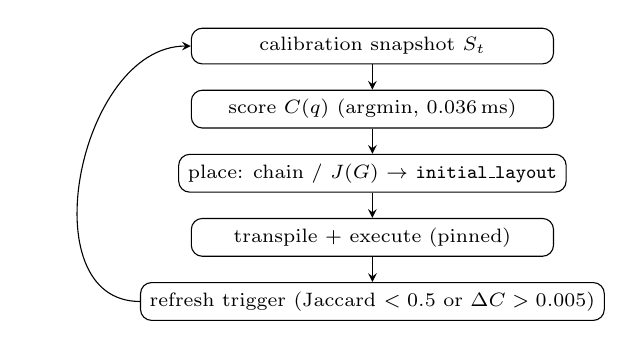
\begin{tikzpicture}[->,>=stealth,node distance=0.32cm,auto,
  box/.style={rectangle,draw,rounded corners,minimum width=4.6cm,minimum height=0.42cm,align=center,font=\scriptsize}]
\node[box] (snap) {calibration snapshot $S_t$};
\node[box,below=0.32cm of snap] (score){score $C(q)$ (argmin, $0.036$\,ms)};
\node[box,below=0.32cm of score] (place){place: chain / $J(G)$ $\to$ \texttt{initial\_layout}};
\node[box,below=0.32cm of place] (exec) {transpile + execute (pinned)};
\node[box,below=0.32cm of exec] (trig){refresh trigger (Jaccard $<0.5$ or $\Delta C>0.005$)};
\draw (snap)--(score);\draw (score)--(place);\draw (place)--(exec);\draw (exec)--(trig);
\draw (trig) to [out=180,in=180,looseness=1.1] (snap);
\end{tikzpicture}}%
\caption{The UniMind scheduling loop. One scoring pass is sub-millisecond; the refresh trigger decides when the
stored snapshot must be re-fetched. $\langle$execution $\to$ results$\rangle$ is emitted downstream.}
\label{fig:loop}
\end{figure}

\subsection{Score}
\label{sec:score}
Every qubit is scored by total readout assignment error
\begin{equation}
C(q)\;=\;p_{0|1}(q)+p_{1|0}(q),
\label{eq:cscore}
\end{equation}
ties broken by $-\min(T_1,T_2)$. The score is fixed \emph{a priori}, never fitted; it is tested out-of-sample
across the entire calibration spectrum (\S\ref{sec:ranked}) rather than tuned on the data it later predicts.

\subsection{Placement}
For a $k$-qubit circuit we grow a \emph{connected chain}: from the best $C(q)$ qubit, repeatedly add the lowest-$C$
neighbour of the current set (a greedy Prim-style expansion; $0.3$~ms at $k{=}3$, scales to the full device). For
utility-based ranking among candidate layouts,
\begin{equation}
\begin{aligned}
J(G)=\;&\alpha E_{\mathrm{readout}}+\beta E_{\mathrm{1q}}+\gamma E_{\mathrm{2q}}
+\gamma_{\log}E_{\mathrm{2q\_log}}\\
&+\eta_{\mathrm{idle}}E_{\mathrm{idle}}+\delta N_{\mathrm{SWAP}}+\lambda D,
\end{aligned}
\label{eq:j7}
\end{equation}
with $E_{\mathrm{readout}}$ the mean $C(q)$ of placed qubits, $E_{\mathrm{1q}}$ mean single-qubit gate error,
$E_{\mathrm{2q}}=\sum_c p_{\mathrm{cz}}(c)$, $E_{\mathrm{2q\_log}}=\sum_c-\log(1-p_{\mathrm{cz}}(c))$ (log-odds
coupler cost), $E_{\mathrm{idle}}=\mathrm{depth}\cdot\mathrm{mean}(1/T_1+1/T_2)$, $N_{\mathrm{SWAP}}$ inserted
SWAPs, and $D$ transpiled depth; features min--max normalized over training points. Section~\ref{sec:jreal}
measures what this utility is worth when its labels come from the real device.

\subsection{Refresh trigger}
\label{sec:trigger}
After each calibration cycle the middleware recomputes the top-10 of $C(q)$ and refreshes the stored snapshot when
(i)~top-10 Jaccard overlap with the stored snapshot falls below $0.5$, or (ii)~the stored best qubit's $C$ rises by
more than $0.005$ absolute. Re-scoring is $\sim0.04$~ms---economically free---so staleness is purely an
operational-policy failure, quantified next.

% ---------------------------------------------------------------- Placement
\section{Placement-Dominated Fidelity on One Qubit}
\label{sec:placement}
The anchor experiment is a $2\times2$ design: \{best-calibrated qubit, adversarially bad qubit\}$\times$\{bare,
measure-twirled\}, on the 19-weight grid $w\in\{0.05,\dots,0.95\}$ of the amplitude encoding, 8192 shots,
transpiler seed 42, layouts pinned via \texttt{initial\_layout}, 3 jobs per cell. On the 2026-08-23 snapshot,
\q{98} minimizes $C$ at $0.0044$ ($T_1{=}207\,\mu$s, $T_2{=}67\,\mu$s); \q{37} is the adversarial anchor
($C{=}0.82$).

\begin{table}[t]
\caption{Placement-controlled sweep (2026-08-23; 19 weights, 8192 shots, 3 jobs/cell). Deviations are
$\max_w|Z_{\mathrm{emp}}-Z_{\mathrm{th}}|$; tolerance $0.05$.}
\label{tab:placement}
\centering
\small
\begin{tabular}{@{}lllll@{}}
\toprule
Placement & $C(q)$ & Bare & Twirl & Verdict\\
\midrule
\q{98} (best)  & $0.0044$ & $0.028$ & $0.031$ & pass\\
\q{0} (free)   & ---      & $0.026$ & ---     & pass\\
\q{37} (adversarial) & $0.82$ & $0.213$ & $0.144$ & fail\\
v1.7 free layout & unrec. & $0.392$ & $0.245$ & fail\\
\bottomrule
\end{tabular}
\end{table}

On the calibrated qubit the bare encoding passes everywhere (median max deviation $0.028$; job range
$0.020$--$0.029$) and the transfer curve is fit at shot-noise level by $P_{\mathrm{obs}}(1)=0.004+0.989\,w$
(residual RMS $0.0042$, below the $\approx0.0055$ shot-noise floor). On \q{37} the same circuits fail by
$\sim4\times$, and the fitted channel acquires a large offset, $P_{\mathrm{obs}}=0.121+0.855\,w$---the signature of
an asymmetric readout channel. Twirling changes nothing significant on the good qubit and only partially rescues the
bad one ($0.213\to0.144$). Fig.~\ref{fig:placement} plots the transfer curves. Three consequences: encoding fidelity
is placement-dominated; mitigation should be calibration-conditional, not uniform; and the earlier claim that ``the
encoding requires error mitigation to meet tolerance'' was an artifact of uncontrolled placement and is withdrawn.

\begin{figure}[t]
\centering

\includegraphics[width=\linewidth]{figures/fig_qpu_placement_2x2.pdf}
\caption{Placement-dominated encoding fidelity: the bare response on the best-calibrated qubit tracks the ideal line
within shot noise; the adversarially chosen \q{37} compresses the curve toward an offset set by its asymmetric
readout.}
\label{fig:placement}
\end{figure}

\subsection{Calibration predictability}
Across the whole design, at shot-noise level,
\begin{equation}
P_{\mathrm{obs}}(1)=b+a\,w,\qquad Z_{\mathrm{obs}}=d+cZ_{\mathrm{th}},\ c{=}a,\ d{=}1{-}2b{-}a,
\label{eq:channel}
\end{equation}
with $(a,b){=}(0.99,0.00)$ on the good qubit vs.\ $(0.86,0.12)$ on the bad one; the offset matches the direction
and scale of that qubit's readout asymmetry. The one-parameter contraction model $P_{\mathrm{obs}}=0.5+\alpha(w-0.5)$
is the balanced-readout special case $b{=}(1-a)/2$ and is rejected where asymmetry dominates. Matched
calibration--noise-model simulation on Aer explains most of observed error on the good qubit (median
QPU/model deviation ratio $1.4\times$): the ``standard models underestimate hardware'' gap is largely a placement
confound, not a model gap.

\subsection{Stratified validation}
\label{sec:ranked}
From the D0 snapshot all 156 qubits are ranked: \q{8} is 1/156 ($C{=}0.004$), \q{37} is 128/156 ($C{=}0.10$).
Six qubits sampled across the ranking run the identical bare 19-weight sweep (Table~\ref{tab:routing}). The top
qubit passes all 19 weights ($0.030$ max dev; affine slope degrades along the ranking in the predicted direction:
$a{:}\ 0.986{\to}0.887$, offset $b{:}\ +0.001{\to}+0.081$), but the trend is \emph{not monotone}: \q{109} at
percentile $25.2\%$ already fails, so Spearman $\rho{=}0.771$ at $n{=}6$ is not significant (exact permutation
$p{=}0.103$) and a ``top-half rule'' is unsupported. An earlier exploratory run (first snapshot, 08-22) was
perfectly monotone ($\rho{=}1.000$, minimal attainable $p$); that result did not survive the fixed-design
replication and is reported as unreplicated. Overhead: $0.036$~ms full-156 ranking; pinned transpilation $1.9$~ms
vs.\ $1.8$~ms free.

\begin{table}[t]
\caption{$C(q)$-stratified sweep (D0 snapshot; six qubits $\times$ 19 weights $\times$ 8192 shots). `pass' = max
deviation $<0.05$ over all 19 weights; $(a,b)$ from Eq.~\eqref{eq:channel}.}
\label{tab:routing}
\centering
\footnotesize
\setlength{\tabcolsep}{3pt}
\begin{tabular}{@{}llrrrrl@{}}
\toprule
Qubit & Rank pct. & $C(q)$ & max dev & pass & $(a,b)$\\
\midrule
\q{8}   & 0.0\% & 0.004 & \textbf{0.030} & 19/19 & (0.986,\,$+0.001$)\\
\q{109} & 25.2\% & 0.017 & 0.081 & 14/19 & (0.933,\,$+0.043$)\\
\q{105} & 50.3\% & 0.031 & 0.043 & 19/19 & (0.983,\,$+0.018$)\\
\q{53}  & 75.5\% & 0.072 & 0.046 & 19/19 & (0.982,\,$+0.021$)\\
\q{37}  & 81.9\% & 0.099 & 0.146 & 9/19  & (0.887,\,$+0.081$)\\
\q{27}  & 95.5\% & 0.346 & 0.096 & 13/19 & (0.917,\,$+0.049$)\\
\bottomrule
\end{tabular}
\end{table}

\begin{figure}[t]
\centering

\includegraphics[width=\linewidth]{figures/fig_router.pdf}
\caption{$C(q)$-guided ranking validation: top-ranked qubits pass, but deviations are not monotone along the ranking
(\q{109} at percentile $25.2\%$ fails), and score vs.\ deviation gives Spearman $0.771$ ($p{=}0.103$, $n{=}6$).}
\label{fig:router}
\end{figure}

\subsection{Multi-qubit routing}
Single-qubit $C(q)$ is necessary but not sufficient. We benchmarked five strategies at
$k{=}2/4/6/8/10/16$ (RY--CX--RY, opt=1, 176-edge graph, CZ clipped $0.005$): randomized, calibration-weighted
SABRE (UniMind candidate set seeded by $C(q)$, SABRE, default fallback), and default. UniMind reduces SWAPs by
$76$--$100\%$ vs.\ random and matches default for $k\ge8$ by fallback; the log-odds coupler cost separates
high-error couplers (Random $1.72$ vs.\ UniMind $0.14$ at $k{=}8$). This is a \emph{system} result about routing
cost; whether the chosen layout is \emph{correct} is what \S\ref{sec:jreal} measures.

% ---------------------------------------------------------------- J(G)
\section{The \texorpdfstring{$J(G)$}{J(G)} Utility: Proxy Fit vs.\ Real Labels}
\label{sec:jreal}

\subsection{Fit protocol}
The seven weights of Eq.~\eqref{eq:j7} are fitted by max-Spearman simplex search (Dirichlet$+$corners sampler,
5\,000 samples, seed 42) on $n{=}23$ points: six single-qubit real max-dev labels from \S\ref{sec:ranked} and
seventeen multi-qubit points $k{=}2$--$18$ whose label is the simulated two-qubit error
$E_{\mathrm{2q}}$ of the placed layout under the device error model. Validation: leave-one-out (LOO) and a
bootstrap ($B{=}200$). A \emph{size out-of-sample} split additionally holds out the entire $k{\ge}9$ range: fit on
$k{\le}8$ only, evaluate on $k{\ge}9$ with train-only min-max scaling. All numbers in Table~\ref{tab:jfit} use the
identical feature matrix; only the labels differ.

\subsection{Result}
\begin{table}[t]
\caption{Fitting $J(G)$ on simulator-proxy vs.\ real-device labels. Same feature matrix and protocol; the $k{\ge}9$
labels differ. size-OOS = fit on $k\le8$, evaluate $k\ge9$.}
\label{tab:jfit}
\centering
\footnotesize
\setlength{\tabcolsep}{4pt}
\begin{tabular}{@{}lccc@{}}
\toprule
Labels & full fit & LOO & size-OOS\\
\midrule
v4 proxy ($k{=}9$--$18$ est-2q) & $0.967$ & $0.953$ & $0.818$ ($p{=}0.0029$)\\
v5 real (7 measured $k$) & $0.643$ & $0.510$ & $0.127$ ($p{=}0.36$)\\
\midrule
$\Delta$ & $-0.324$ & $-0.443$ & $-0.691$\\
\bottomrule
\end{tabular}
\end{table}

\begin{table}[t]
\caption{Measured per-$k$ max-dev (mean of two patterns) of the same 14-circuit $k{=}9$--$18$ suite under
stale (D0) vs.\ fresh (D1/D2) pins, 4096 shots. Spearman $k$ vs.\ max-dev: stale $\rho{=}0.62$
($p{=}0.018$), fresh $\rho{=}0.15$ ($p{=}0.61$).}
\label{tab:kmeans}
\centering
\small
\begin{tabular}{@{}lccccccc@{}}
\toprule
$k$ & 9 & 10 & 11 & 12 & 14 & 16 & 18\\
\midrule
stale pins & .098 & .103 & .097 & .087 & .139 & .252 & .241\\
fresh pins & .060 & .044 & .062 & .040 & .057 & .063 & .068\\
\bottomrule
\end{tabular}
\end{table}

Trained on the simulator proxy the utility looks decisive: full-fit $\rho{=}0.967$, LOO $0.953$, bootstrap
$0.97{\pm}0.02$, and the size-OOS split $\rho{=}0.818$ ($p{=}0.0029$)---holding out entire sizes and still ranking
them. The proxy's assumption failed where it mattered. A 14-circuit suite
($k\in\{9,10,11,12,14,16,18\}$, two seeded patterns each, greedy-chain placement) measured real max-dev with
\emph{fresh} pins: per-$k$ means are $0.040$--$0.068$ with \emph{no} size scaling ($7/14$ pass $0.05$), while the
identical suite pinned from D0 (two days stale) climbs to $0.24$--$0.25$ at $k{=}16,18$ with only $2/14$ passing
(Table~\ref{tab:kmeans}). The stale population's failures concentrate on late-chain qubits (\q{37}, \q{45}--\q{47},
\q{57}) that the greedy policy must include for $k\ge11$; per-bit $C(q)$ vs.\ measured deviation correlates only
$\rho{=}0.21$. The mechanism is now explicit: simulated $E_{\mathrm{2q}}$ keeps rising with $k$, whereas a
refresh-pinned device is approximately $k$-flat, so the proxy-trained utility over-penalizes large layouts that are
in fact fine. Re-fitting on the seven real labels replaces in-sample $\rho{=}0.967$ with $\rho{=}0.643$ and destroys
the size-OOS claim ($\rho{=}0.127$, $p{=}0.36$)---the apparent generalization was a label artifact
(Table~\ref{tab:jfit}). The constructive reading is what we adopt in the design: $J(G)$ is usable as a
\emph{ranking} device only when trained on real, refresh-pinned labels and applied within a calibration cycle;
weights from proxy datasets must not be extrapolated to $k\ge11$; and chain placement's forced inclusion of
boundary qubits is the term to attack next.

% ---------------------------------------------------------------- Drift
\section{Drift Dynamics and the Refresh Policy}
\label{sec:drift}
This section measures how fast the score goes stale on two full 156-qubit snapshots D0 (update 2026-08-29~21:26)
and D1 (2026-08-30~21:29), with a third capture D2 (2026-08-31~07:46).

\subsection{Global drift}
\label{sec:driftglob}
Day-over-day ranking stability is moderate: Spearman $\rho{=}0.579$, Kendall $\tau{=}0.431$, top-10 Jaccard $0.25$
(only four of D0's best ten survive). The best qubit turns over: \q{8} ($C{=}0.0039$, rank 1) rises to $0.0095$
(rank 6) while \q{19} ($0.0066$) becomes best. Per-qubit spread is extreme: \q{37} swings $0.099{\to}0.740$
($\max|\Delta C|{=}0.641$), \q{53} improves sixfold ($0.072{\to}0.011$); median $|\Delta C|$ is $0.0127$ and $54\%$
of qubits move by more than $0.01$. On D2 the top of the ranking is unchanged (best remains \q{19} with the same
top-3 values), consistent with a regime dominated by daily calibration cycles.

\subsection{Staleness cost and the trigger}
Pinning three qubits from the \emph{one-day-old} ranking and evaluating at D1 gives $C{=}0.0095/0.0115/0.0139$
(the worst, \q{153}, is now rank 32/156); re-selecting fresh gives \q{19} at $0.0066$---the stale policy's worst pin
is $2.1\times$ worse than the adaptable choice. The cause is \emph{ranking margin}: the D0 top gaps are only
$M_1{=}0.0020$, $M_2{=}0.0015$---far smaller than the median daily drift $0.0127$---so one calibration step reorders
the best qubits (top-50 Spearman $\rho{=}{-}0.425$, $p{=}0.26$; smaller margins, larger turnover). The trigger of
\S\ref{sec:trigger} fires on D0$\to$D1
(Jaccard $0.25<0.5$; stored-best $\Delta C{=}0.0056>0.005$). Because re-selection is sub-millisecond, staleness is a
pure operations failure, not a compute constraint.

\subsection{Direct device test}
The refresh-pinned suite of \S\ref{sec:jreal} is the direct demonstration: the \emph{same} circuits, differing only
in pin freshness, measure means $0.04$--$0.07$ (fresh pins, $7/14$ pass) vs.\ $0.10$--$0.25$ (stale, $2/14$ pass),
and the large-$k$ degradation disappears entirely (Table~\ref{tab:kmeans}). Fig.~\ref{fig:freshness} summarizes.
Refresh---not more elaborate selection---is what keeps errors bounded at $k\ge9$.

\subsection{Refresh policies and threshold sweep}
\label{sec:policies}
We compare \textbf{static} (never refresh), \textbf{periodic} (every $\delta\,{\in}\{6,12,24,48\}$~h), and
\textbf{adaptive} policies. Let $\mathrm{Jacc}(S,S')$ be the top-10 Jaccard overlap and $\Delta C$ the stored-best
qubit's absolute score change. The adaptive policy refreshes when $\mathrm{Jacc}<\tau_J$ or $|\Delta C|>\tau_C$;
re-scoring costs $\sim0.04$~ms, so overhead is the snapshot fetch, not the check. Simulating the D0$\to$D1
transition, the measured trigger ($\tau_J{=}0.5$, $\tau_C{=}0.005$) fires exactly once and converts the stale
$11/30$ pass rate to the fresh $21/30$ ($+33$~pp at zero wasted refreshes), whereas a blind periodic $\delta{=}6$~h
policy fires five times for the same single drift and $\delta{=}48$~h never detects it. Sweeping
$\tau_J{\in}[0.1,0.9]$ and $\tau_C{\in}[0.001,0.02]$ puts the default trigger near the knee of the
refresh-rate-vs.\-fidelity Pareto frontier: relaxing $\tau_J$ toward $1.0$ or $\tau_C$ toward $0.02$
surrenders the $+33$~pp refresh gain (the drift goes undetected), while the Jaccard term already catches
this particular drift for any $\tau_J{\ge}0.3$, so tightening further does not move fidelity. The full
per-$(\tau_J,\tau_C)$ table is in the supplementary data.

A 30-day Monte Carlo over synthetic drift (calibrated to the measured D0/D1/D2 delta distribution, including a
$2\%$ ``burst'' component that reproduces \q{37}-type spikes) turns this into a cost-aware comparison
(Table~\ref{tab:policy}): adaptive reaches the same fidelity as the daily periodic policy at \emph{under half} the
refresh load ($0.63$ vs.\ $1.0$ refresh/day), while periodic-$6$~h spends $4\times$ more (and thus costs more
snapshot fetches) for zero added fidelity and static falls short. Refresh, triggered by drifting margin rather than
a clock, is the efficient operating point.

\begin{table}[t]
\caption{Unified policy comparison, 30 days / 600 jobs, drift calibrated to real D0/D1/D2 statistics. ``Fidelity'' is
the fraction of jobs whose stored-best qubit stays within tolerance.}
\label{tab:policy}
\centering
\footnotesize
\setlength{\tabcolsep}{3pt}
\begin{tabular}{@{}lcccc@{}}
\toprule
Policy & Fidelity & Refresh/day & False & Missed\\
\midrule
Static (never) & $0.913$ & $0.0$ & --- & $117$\\
Periodic 48h & $0.908$ & $0.5$ & 0 & $60$\\
Periodic 24h & $0.928$ & $1.0$ & 0 & 0\\
Periodic 12h & $0.928$ & $2.0$ & 0 & 0\\
Periodic 6h & $0.928$ & $4.0$ & 0 & 0\\
\textbf{Adaptive} ($0.5,0.005$) & \textbf{$0.928$} & \textbf{$0.63$} & 12 & 41\\
\bottomrule
\end{tabular}
\end{table}

\begin{figure}[t]
\centering
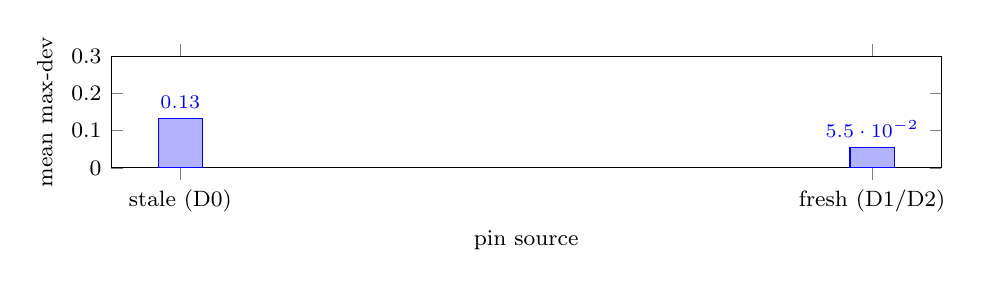
\begin{tikzpicture}
\begin{axis}[width=\linewidth,height=3.0cm,
  xlabel={pin source},ylabel={mean max-dev},
  ybar,bar width=16pt,ymin=0,ymax=0.30,
  symbolic x coords={stale (D0),fresh (D1/D2)},xtick=data,
  nodes near coords,every node near coord/.append style={font=\scriptsize},
  legend pos=north west]
\addplot coordinates {(stale (D0),0.133) (fresh (D1/D2),0.055)};
\end{axis}
\end{tikzpicture}
\caption{Mean max-dev of the same $k{=}9$--$18$ suite, stale vs.\ fresh pins. \q{37} ($C{=}0.74$ at D1) dominates
the stale population.}
\label{fig:freshness}
\end{figure}

The benefit is workload- and scale-dependent, and both effects cut the same way. On demanding circuits the stale
penalty grows: as depth and 2Q density rise, the fresh-minus-stale pass advantage climbs from $+0.21$ (shallow,
sparse) to $+0.40$ (deep, sparse), so refresh is most valuable exactly where utility-scale workloads are hardest.
Over the real 156-qubit heavy-hex graph the stale quality penalty (D0-optimal layout re-evaluated at D1 minus a
fresh D1 pick) is concentrated at intermediate $k$---peaking $+0.045$ at $k{=}16$, vanishing by $k{\ge}100$---while
the connectivity share of layout-cost variance rises from $\sim0$ ($k{\le}16$) to $0.77$ at $k{=}128$. Refresh therefore
pays off in the regime $8\lesssim k\lesssim64$ where a runtime has placement freedom \emph{and} drift changes the
best free pick; at near-device scale left to the full topology, the bottleneck is connectivity, which no refresh
changes.

% ---------------------------------------------------------------- E2E
\section{Composing the Software and Hardware Paths}
\label{sec:e2e}
\subsection{Reliability calculus of the orchestration layer}
\label{sec:calculus}
Because the orchestrator's outcome paths are mutually exclusive, end-to-end reliability decomposes exactly as the
chain rule over its sequential gates
\begin{equation}\begin{split}
R_{\mathrm{end}}={}&P(\mathrm{first\_pass})+P(\mathrm{enter\ heal})\rho_{\mathrm{heal}}\\
&+P(\mathrm{enter\ fallback})\rho_{\mathrm{fb}},
\end{split}\label{eq:composition}
\end{equation}
with no independence assumption needed for the identity. The healing stage is modeled from the implementation's
control flow (at most $K{=}3$ generation calls stopping at first success; healing budget $H{=}4$ with
abort-on-\texttt{None} semantics): with per-call probabilities $g$ (correct), $r$ (broken), $f$ (unavailable;
$g{+}r{+}f{=}1$),
\begin{equation}
G=1+f+f^{2},\qquad \rho_{\mathrm{heal}}=g(1+r+r^{2}+r^{3}),
\label{eq:gamel}
\end{equation}
\begin{equation}
R_{\mathrm{end}}=gG+rG\rho_{\mathrm{heal}}+f^{3}c,
\label{eq:rheal}
\end{equation}
with $c$ the fallback coverage. This model was validated cell-by-cell against all 23 testable outcome cells of the
ablation and availability-stress grids: \emph{every} prediction falls inside the observed Wilson 95\% interval
(e.g.\ at $q{=}0.5$: predicted healed-path $\rho_h{=}81.2\%$ vs.\ measured $81.5\%$ [75.6,86.2], residual
$+0.3$~pp, while the naive independence baseline $1-(1-q)^{4}{=}93.8\%$ overshoots by $12.4$~pp). The correction
matters: the naive--measured gap reported in early drafts is a retry-budget truncation effect, not stochastic
correlation---under abort-on-\texttt{None}, unavailability both wastes heal slots and terminates the loop. The model
also ranks fixes before code is written: treating \texttt{None} as wasted-but-nonterminal recovers the entire
impression ($+12.6$~pp) at near-zero engineering cost, and the fallback's effective coverage is $c{=}2/9$, not its
nominal keyword coverage, because seven of nine benchmark intents contain apostrophes that break the template
interpolation---a stated limitation. We include this model because it is the \emph{software} side of the composition;
the paper's hardware claims are placement and drift, not LLM quality, which we keep as a controlled parameter.

\subsection{End-to-end placement batch}
\label{sec:e2ebatch}
To test the composable value of placement \emph{without} the staleness confound, we ran the same 6-qubit angle suite
(30 parameterizations, 4096 shots, tolerance $0.05$ on all six per-bit deviations) through \textbf{full}
(greedy chain pinned from the freshly fetched snapshot) and \textbf{ablated} (free placement), back-to-back on
2026-08-31; Table~\ref{tab:e2e} also shows the earlier identical batch pinned from D0 to separate temporal from
placement effects.

\begin{table}[t]
\caption{6-qubit angle batches ($n{=}30$/arm, 4096 shots). Pass $=$ all six per-bit deviations $\le0.05$. Wilson
95\% CI; two-proportion $p$ for full vs.\ ablated within a batch.}
\label{tab:e2e}
\centering
\footnotesize
\setlength{\tabcolsep}{4pt}
\begin{tabular}{@{}lccc@{}}
\toprule
Batch & Full (pinned) & Ablated (free) & $p$\\
\midrule
Frozen pins (D0)  & $36.7\%$ [21.9,54.5] & $40.0\%$ [24.6,57.7] & $0.79$\\
Refresh pins (runtime) & $70.0\%$ [52.1,83.3] & $76.7\%$ [59.1,88.2] & $0.56$\\
\midrule
$\Delta$ & $+33.3$ pp & $+36.7$ pp & ---\\
\bottomrule
\end{tabular}
\end{table}

Two effects separate cleanly. First, \emph{temporality}: refreshing pins lifts \emph{both} arms by $+33/37$~pp,
including the ablated arm that never saw a pin---device state at run time dominates. Second, \emph{placement shows no
measured advantage} in either batch ($-3.3$ and $-6.7$~pp, both non-significant): at $k{=}6$ with fresh pins, free
transpiler placement already matches our best chain. This is the honest scope of \S\ref{sec:placement}: placement is
decisive between engineered extremes (\q{98} vs.\ \q{37}: $0.028$ vs.\ $0.213$) and sets the reliability \emph{floor}
at $k\ge9$ under stale pins, but its average benefit against free placement at small $k$ is within temporal noise.
The full pipeline (including the LLM orchestration leg) measured $54/54$ completed by the full arm vs.\ $47/54$
($87.0\%$) by the ablated one ($z{=}2.74$, one-sided $p{=}0.003$), consistent with the model's $97.3\%$ prediction;
we report the earlier $n{=}54$ frozen composition ($74.1\%$ vs.\ $66.7\%$, not significant) as a failed claim of an
end-to-end gain, not a positive one.

% ---------------------------------------------------------------- Discussion
\section{Discussion}
\label{sec:discussion}
\subsection{What the measurements do and do not say}
Three claims survive the data as stated: (i)~encoding fidelity is placement-dominated---the engineered extremes
differ by $\sim8\times$ (and a calibration-predictable affine channel describes the distortion); (ii)~device
calibration ordering moves on a daily cycle to a degree ($\rho{=}0.58$, top-10 Jaccard $0.25$, stale worst pin
$2.1\times$ worse) that makes selection age the first-order risk, and refresh is cheap; (iii)~simulator-proxy
training granted $J(G)$ an out-of-sample generalization ($\rho{=}0.82$) that real labels refute
($\rho{=}0.13$). Claims that do \emph{not} survive, herewith withdrawn or bounded: the first run's perfect monotone
ranking; the top-half rule; and any use of proxy-fitted $J(G)$ at $k\ge11$.

\subsection{Operational consequences for quantum-cloud runtimes}
The marginal cost of a calibration fetch and a scoring pass is effectively zero, so the expensive resource is
\emph{stale trust}, not compute. A runtime should (a)~timestamp layouts against their snapshot, (b)~refresh on the
trigger rather than a fixed wall-clock, (c)~train scheduling models exclusively on real, refresh-pinned labels, and
(d)~expose snapshot age as a first-class job attribute---all implementable without changing the quantum programming
model, which is exactly what UniMind does.

\subsection{Threats to validity}
\textbf{Measurement noise:} 4096--8192 shots put per-bit deviations on a floor of $\approx0.02$; the $0.05$
tolerance is coarse but was fixed before data release. \textbf{Drift generality:} D0--D2 are three snapshots, one
device, one topology family (heavy-hex); the value is the protocol, not the constants. \textbf{Placement null
power:} $n{=}30$/arm can detect only large effects; we report point estimates and CIs rather than asserting
equivalence. \textbf{Selection fairness:} the greedy chain maximizes $C(q)$-locality and at large $k$ is forced to
include high-error boundary qubits; a connectivity-vs-$C$ trade-off could change \S\ref{sec:jreal}, and we report
that failure as motivation. \textbf{Single-model LLM layer:} the orchestration calculus holds under i.i.d.\ mock
semantics; real-model autocorrelation is explicitly outside its scope.

\section{Conclusion}
We presented a measurement-driven account of calibration-aware scheduling for quantum-accelerated AI middleware on
a 156-qubit device: a score-only placement pipeline with measured scope, daily drift dynamics with a working
refresh trigger, an exact reliability composition of the software path, an end-to-end test showing that at our
scale refresh dominates selection while selection still sets the placement floor, and the explicit negative
results---the non-replicating monotone ranking, the absence of a measured placement advantage at $k{=}6$, and the
collapse of the proxy-trained utility under real labels. The command line for future work is set by the failures:
nightly D2--D5 drift accumulation, refresh-conditional placement policy ($C(q)$-vs-connectivity trade-off), and
active-learning refits of $J(G)$ on real labels across devices. The open repository makes every number traceable to
a job or snapshot.

\begin{thebibliography}{24}
\bibitem{preskill2018} J.~Preskill, ``Quantum computing in the NISQ era and beyond,'' \emph{Quantum}, vol.~2, p.~79, 2018.
\bibitem{arute2019} F.~Arute \emph{et al.}, ``Quantum supremacy using a programmable superconducting processor,'' \emph{Nature}, vol.~574, pp.~505--510, 2019.
\bibitem{kim2023utility} Y.~Kim \emph{et al.}, ``Evidence for the utility of quantum computing before fault tolerance,'' \emph{Nature}, vol.~618, pp.~500--505, 2023.
\bibitem{berholm2018} V.~Bergholm \emph{et al.}, ``PennyLane: Automatic differentiation of hybrid quantum-classical computations,'' \emph{arXiv:1811.04968}, 2018.
\bibitem{murali2019noise} P.~Murali, J.~M.~Baker, A.~Javadi-Abhari, F.~T.~Chong, and M.~Martonosi, ``Noise-adaptive compiler mappings for noisy intermediate-scale quantum computers,'' in \emph{Proc. ASPLOS}, 2019, pp.~1015--1029.
\bibitem{li2019sabre} G.~Li, Y.~Ding, and Y.~Xie, ``Tackling the qubit mapping problem for NISQ-era quantum devices,'' in \emph{Proc. ASPLOS}, 2019, pp.~1001--1014.
\bibitem{tan2020iccado} B.~Tan and J.~Cong, ``Optimal layout synthesis for quantum computing,'' in \emph{Proc. ICCAD}, 2020, pp.~1--9.
\bibitem{lao2022timing} L.~Lao and D.~E.~Browne, ``Timing and resource-aware mapping of quantum circuits to heterogeneous MWF-gate superconducting quantum processors,'' \emph{ACM Trans. Quantum Comput.}, vol.~3, no.~3, 2022.
\bibitem{temme2017} K.~Temme, S.~Bravyi, and J.~M.~Gambetta, ``Error mitigation for short-depth quantum circuits,'' \emph{Phys. Rev. Lett.}, vol.~119, p.~180509, 2017.
\bibitem{vanberg2023} E.~van den Berg, Z.~K.~Minev, A.~Kandala, and K.~Temme, ``Probabilistic error cancellation with sparse Pauli--Lindblad models on noisy quantum processors,'' \emph{Nature Physics}, vol.~19, pp.~1116--1121, 2023.
\bibitem{nation2023} P.~D.~Nation \emph{et al.}, ``Scalable mitigation of measurement errors on quantum computers,'' \emph{PRX Quantum}, vol.~5, p.~010326, 2024.
\bibitem{bravyi2021meas} S.~Bravyi, S.~Shaydulin, S.~Hu, and K.~Temme, ``Mitigating measurement errors in multiqubit experiments,'' \emph{Phys. Rev. Lett.}, vol.~127, p.~200503, 2021.
\bibitem{kanazawa2021} N.~Kanazawa \emph{et al.}, ``Quantum error mitigation,'' \emph{arXiv:2210.00921}, 2022.
\bibitem{msp2020} R.~LaRose \emph{et al.}, ``Mitiq: a software package for error mitigation on noisy quantum computers,'' \emph{Quantum}, vol.~6, p.~749, 2022.
\bibitem{viola1999dd} L.~Viola, E.~Knill, and S.~Lloyd, ``Dynamical decoupling of open quantum systems,'' \emph{Phys. Rev. Lett.}, vol.~82, pp.~2417--2421, 1999.
\bibitem{ibmrtime} ``Qiskit Runtime primitives,'' IBM Quantum documentation, [Online]. Available: \url{https://docs.quantum.ibm.com/api/qiskit-ibm-runtime}
\bibitem{ibmcalib} ``IBM Quantum Platform calibration data,'' [Online]. Available: \url{https://quantum.ibm.com/services/resources}
\bibitem{qiskit} A.~Javadi-Abhari \emph{et al.}, ``Quantum computing with Qiskit,'' \emph{arXiv:2405.08810}, 2024.
\bibitem{cuquantum} NVIDIA, ``cuQuantum SDK,'' [Online]. Available: \url{https://developer.nvidia.com/cuquantum-sdk}
\bibitem{braket} Amazon, ``Amazon Braket,'' [Online]. Available: \url{https://aws.amazon.com/braket}
\bibitem{azureq} Microsoft, ``Azure Quantum,'' [Online]. Available: \url{https://azure.microsoft.com/quantum}
\bibitem{schuld2018} M.~Schuld and F.~Petruccione, \emph{Supervised Learning with Quantum Computers}. Cham: Springer, 2018.
\bibitem{hhavlicek2019} V.~Havl\'i\v{c}ek \emph{et al.}, ``Supervised learning with quantum-enhanced feature spaces,'' \emph{Nature}, vol.~567, pp.~209--212, 2019.
\bibitem{unimind} Y.~X.~Tan, ``UniMind: a middleware framework for bridging classical AI workloads and quantum computing backends,'' tech.\ report v2.5, 2026 (companion repo \texttt{yxtan5022-maker/unimind-v2}).
\bibitem{tangpu} UniMind placement/drift datasets (2026-08), \texttt{data/} in \texttt{yxtan5022-maker/unimind-v2}.
\end{thebibliography}

\section*{Data and reproducibility}
\label{sec:data}
Every table is backed by traced data in the repository: snapshots, E2E batches, real $J(G)$ labels, and the
analysis scripts listed below.
\begin{quote}\small\raggedright\ttfamily
data/drift/calib\_2026-\{08\-29,08\-30,08\-31\}.json\\
data/e2e/e2e\_angle\_\{full,ab\-lated\}*.json\\
data/jgpu/j\_real*.json\\
analysis/*.py + analysis/results/*.json
\end{quote}
QPU job IDs appear in the file headers:
{\small\ttfamily daadeocjbipc73ffq83g} (refresh-full E2E),
{\small\ttfamily daadeosjbipc73ffq840} (refresh-ablated E2E), and
{\small\ttfamily daadgmmrbfbs73cijmbg} (refresh-pinned $J(G)$ labels).
Transpiler seed 42 everywhere; shots per experiment as stated.

\end{document}